
% !TEX program = pdflatex
% !TEX enableSynctex = true
% !BIB program = bibtex


\documentclass[12pt]{article}

\usepackage{setspace}
\usepackage{amsmath}
\usepackage{amsfonts}
\usepackage{graphicx}
\usepackage{float}
\addtolength{\oddsidemargin}{-.7in}
\addtolength{\evensidemargin}{-.7in}
\addtolength{\textwidth}{1.4in}
\usepackage{enumerate}
\onehalfspacing
\usepackage{geometry} % Required for customizing page layout

\usepackage{caption}
\usepackage{booktabs}

\usepackage{hyperref}
\hypersetup{
	pdfstartview = FitH,
	pdfauthor = {...},
	pdftitle = {...},
	pdfkeywords = {...; ...; ...; ...},
	colorlinks = true,
	linkcolor = blue,
	urlcolor = blue,
	citecolor = blue,
	linktocpage=true
}


\begin{document}
\section{Partial equilibrium model - VFI only}
\subsection{Ver 1 - PE model - Fixed Qs - 3 state variables}
Productivity process: two-state markov chain \vspace{3mm} \\
Labour policy: 
\begin{equation}
    n(k,\varepsilon_i) = \left( \dfrac{ \nu \varepsilon_i k^\alpha}{w} \right)^{\frac{1}{1-\nu}}
\end{equation}
Corresponding output: 
\begin{equation}
    y(k,\varepsilon_i) = \varepsilon_i k^{\alpha} \left( \dfrac{\nu \varepsilon_i k^\alpha}{w} \right)^{\frac{\nu}{1-\nu}}
\end{equation}
Corresponding profits: 
\begin{equation}
    \pi(k,\varepsilon_i) = (1-\nu) y(k,\varepsilon_i) - c
\end{equation}
External finance premium - just a parameter \vspace{2mm} \\
Value function:
\begin{equation}
     V(k,b, \varepsilon_i) = \max_{k',b'}  \left( \pi(k,\varepsilon_j)+(1-\delta)k - k' +  q^s b' -b  +
            \beta (1-P_\chi) \sum_{j=1}^{N_\varepsilon} g_{ij}  V(x',\varepsilon_j') \right)
\end{equation}
\noindent Here, the firm can directly choose $k'$ and $b'$, which makes coding the transition matrix easier, since you do not have to interpolate the Q-es. In the end you just have some very sparse matrices, since the model is almost deterministic. \vspace{3mm} \\
The shortcoming is you have 3 state variables and 2 action variables, which means that it is very hard to move past a grid size of 30. 

\newpage
\setcounter{equation}{0}


\subsection{Ver 2 - Fixed Qs - cash on hand - two-state productivity}
Productivity process: two-state markov chain \vspace{3mm} \\
Labour policy: 
\begin{equation}
    n(k,\varepsilon_i) = \left( \dfrac{ \nu \varepsilon_i k^\alpha}{w} \right)^{\frac{1}{1-\nu}}
\end{equation}
Corresponding output: 
\begin{equation}
    y(k,\varepsilon_i) = \varepsilon_i k^{\alpha} \left( \dfrac{\nu \varepsilon_i k^\alpha}{w} \right)^{\frac{\nu}{1-\nu}}
\end{equation}
Corresponding profits: 
\begin{equation}
    \pi(k,\varepsilon_i) = (1-\nu) y(k,\varepsilon_i) - c
\end{equation}
Future cash on hand: 
\begin{equation}
   x' = \pi(k',\varepsilon_j')+(1-\delta)k'-b'
\end{equation}
External finance premium 
\begin{equation}
    q^s = 0.94
\end{equation}
Need an equity finance option. Otherwise there certain states are not associated to any feasible action. Here, I assume. This means that firms will sometimes have negative cash on hand. 
\begin{equation}
    d < 0 \implies d = 1.6d
\end{equation}
Value function:
\begin{equation}
     V(x,\varepsilon_i) = \max_{k',b'}  \left(x - k' +  q^s b' + 
            \beta  (1-P_\chi)  \sum_{j=1}^{N_\varepsilon} g_{ij} V(x',\varepsilon_j') \right)
\end{equation}
Adding cash on hand reduces the grid to 2 state and 2 action variables. This implies that you can do a much larger grid. However, you have to interpolate resulting x that follows from choices k' and b' to the grid, since x-here is the result. This could be a problem. Generally, results are well behaved in this case, although they are very mechanical. 


\begin{figure}[H]  % [h] indicates placing the image here
    \centering
    \caption{Ver2 - prod: 5, 8} \label{chart:CFLcdf}
    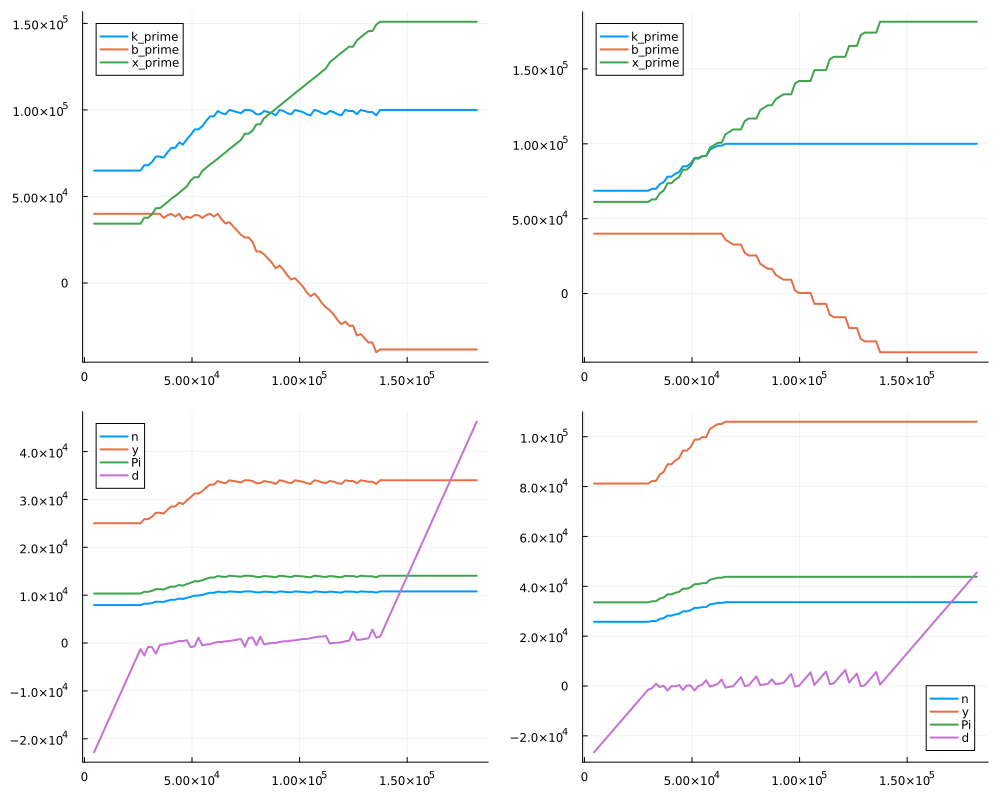
\includegraphics[width=1\textwidth]{ver2.png}
\end{figure}


\newpage
\setcounter{equation}{0}

\subsection{Ver 3 - ABL Qs - cash on hand - AR(1) productivity}
Productivity process: AR(1) process with multiple states. Below, I plot the worst the median and the best productivity state. \vspace{3mm} \\
Labour policy: 
\begin{equation}
    n(k,\varepsilon_i) = \left( \dfrac{ \nu \varepsilon_i k^\alpha}{w} \right)^{\frac{1}{1-\nu}}
\end{equation}
Corresponding output: 
\begin{equation}
    y(k,\varepsilon_i) = \varepsilon_i k^{\alpha} \left( \dfrac{\nu \varepsilon_i k^\alpha}{w} \right)^{\frac{\nu}{1-\nu}}
\end{equation}
Corresponding profits: 
\begin{equation}
    \pi(k,\varepsilon_i) = (1-\nu) y(k,\varepsilon_i) - c
\end{equation}
Future cash on hand: 
\begin{equation}
   x' = \pi(k',\varepsilon_j')+(1-\delta)k'-b'
\end{equation}
External finance premium:
\begin{equation}
    q^{abl}(k',b')b' = \beta \left[ (1-P_\chi) b' + P_\chi \min\{b', \ \phi_k (1-\delta) k' \} \right]  
\end{equation}
Equity finance option:
\begin{equation}
    d < 0 \implies d = 1.6d
\end{equation}
Value function:
\begin{equation}
     V(k,b, \varepsilon_i) = \max_{k',b'}  \left( x - k' +  q^s b' +
            \beta (1-P_\chi) \sum_{j=1}^{N_\varepsilon} g_{ij}  V(x',\varepsilon_j') \right)
\end{equation}
Here the two innovations are that interest rates are endogenous and the productivity process is more realistic. Results makes sense, although they display this jigsaw pattern in certain regions and calibrations. \textbf{Weirdly, the model breaks down when grids are defined logarithmically.} Firms very quickly converge to their desired level of capital, even if they are cash-poor - that is because $q$ remains relatively large even for very indebted firms.

\begin{figure}[H]  % [h] indicates placing the image here
    \centering
    \caption{Ver3 - worst, median and best productivity states} \label{chart:CFLcdf}
    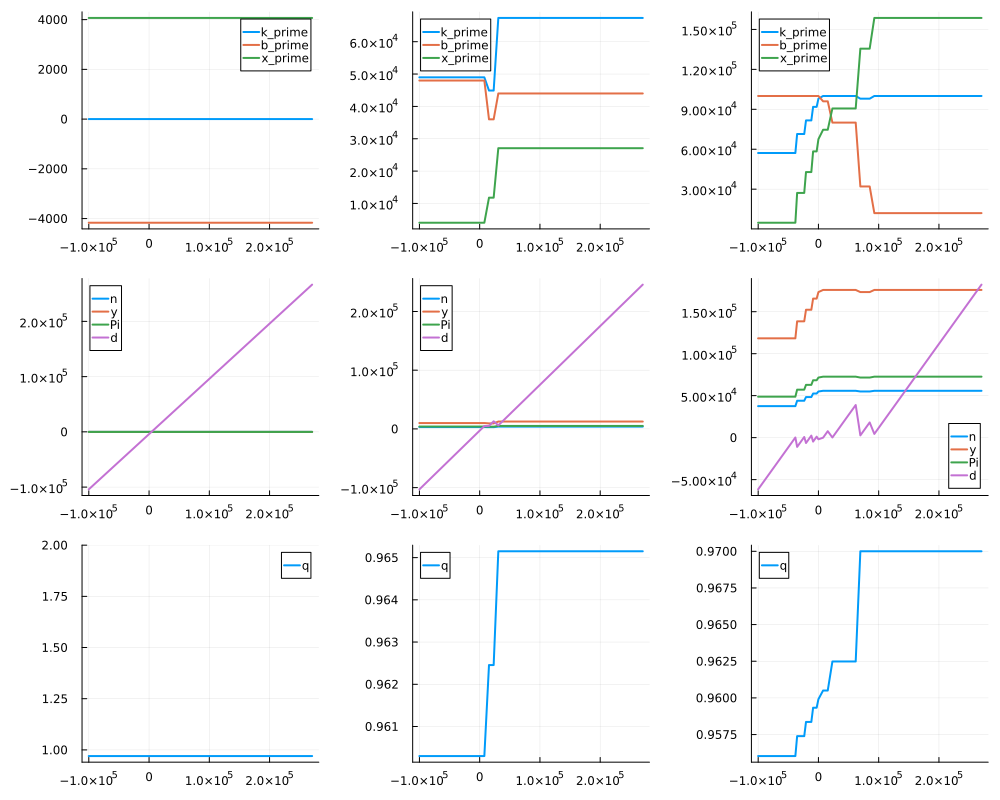
\includegraphics[width=1\textwidth]{ver3.png}
\end{figure}


\newpage

\section{Summary of models up to Ver 3}

Measure of size problem: 
\begin{itemize}
    \item The problem with the cash on hand approach is that it does not have a good measure of current size. The current cash on hand might be misleading since large debt might cancel out large capital stocks.
    \item The best solution is to interpret everything in terms of next period's capital or production. This is ok but only if there is is a proper dispersion of capital stocks.
\end{itemize} 
On interest rates:
\begin{itemize}
    \item One problem with the current calibration is that you see $q$-s that are only marginally smaller than $\beta$. This implies that even poor firms can borrow a lot very quickly and they can jump to optimal capital very quickly. 
    \item The main drivers of interest rates are $\phi_a$ (resale value of capital) and $P_{\chi}$ probability of default. You can try adjusting these, but the effect on overall $q$ will be minimal. 
\end{itemize}
I might have to add default probabilities to the model:
\begin{itemize}
    \item Exogenous approach: default probability is a decreasing function of $x$
    \item Kaas approach: default when there are no feasible actions left for the firm 
    \item C\&D approach: default when the firm sees that the when $-x$ is smaller than the continuation value
    \item Simplified C\&D approach: the firm defaults in future $x$ is negative
\end{itemize}
On debt debt demand of firms
\begin{itemize}
    \item Here firms discount future by $\beta(1-P_\chi)$, whereas the fully secured interest rate is $\beta$. Therefore, when the firms manages to be fully secured, it prefers to hold a lot of debt and pay higher dividends, because if it default next period it won't have to repay this debt
    \item This implies that even large, cash rich companies hold a lot of debt. This is a nice result, that is due to bad assumptions. 
\end{itemize}


\subsection{Ver 4 - Adding endogenous exits to Ver 3}
Productivity process: AR(1) process with multiple states. Below, I plot the worst the median and the best productivity state. \vspace{3mm} \\
Same as in Ver 3: 
\begin{itemize}     \setlength\itemsep{0em}
    \item Labour policy
    \item Corresponding output
    \item Corresponding profits
    \item Future cash on hand
    \item External finance premium
\end{itemize}
Equity finance option
\begin{itemize}
    \item Not necessary anymore, since firms can decide to exit in any state. That being said, this implies that for low cash on hand values the firm must borrow a lot just to avoid exit. 
\end{itemize}
Exit decision: state and action at the same time, if exit decision was made last period the current state is always exit. This is associated with a zero value. If exit decision is made this period the next state is always exit and the current return is: 
\begin{equation}
    exit = 1 \implies d = x \newline \hspace{5mm} or \hspace{5mm}
    exit = 1 \implies d = 0 
\end{equation}
The first one is associated to exit, and the second is closer to default. \vspace{3mm} \\
Value function:
\begin{equation}
     V(k,b, \varepsilon_i) = \max_{k',b'}  \left( x - k' +  q^s b' +
            \beta (1-P_\chi) \sum_{j=1}^{N_\varepsilon} g_{ij}  V(x',\varepsilon_j') \right)
\end{equation}

\begin{figure}[H]  % [h] indicates placing the image here
    \centering
    \caption{Ver4 - exit decisions, no equity finance, no default} \label{chart:CFLcdf}
    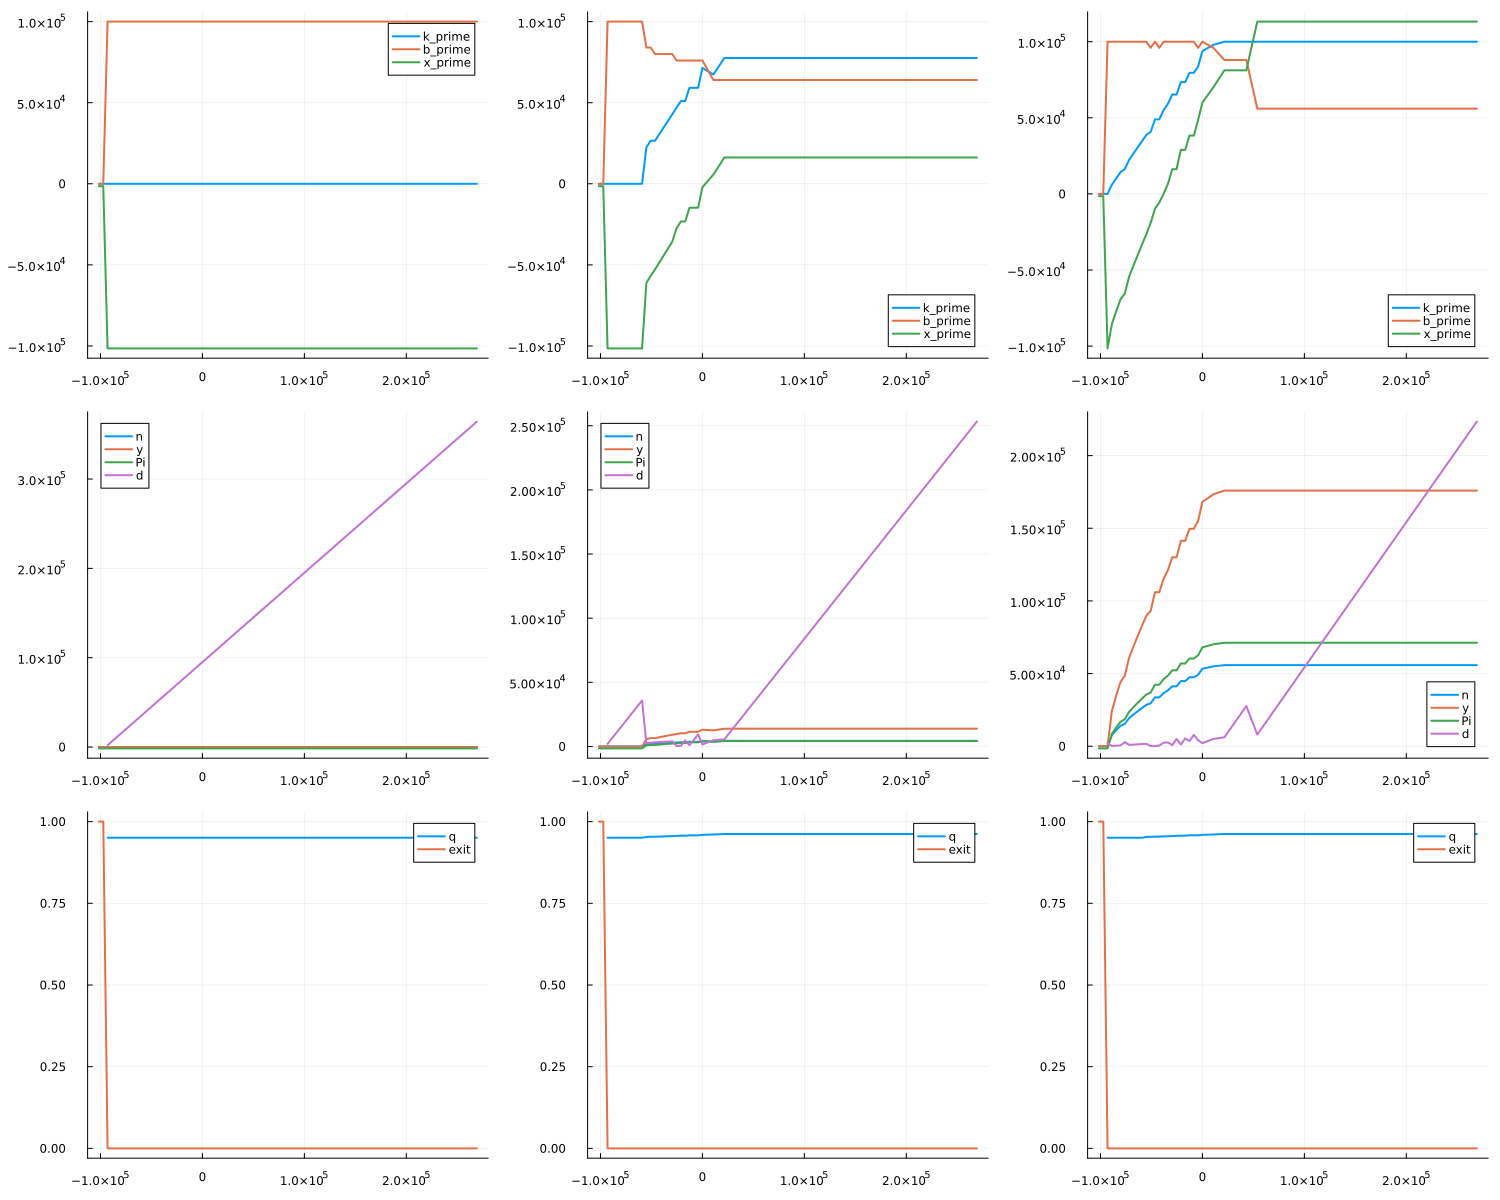
\includegraphics[width=1\textwidth]{ver4.png}
\end{figure}


\end{document}






